\documentclass[11pt]{article}

\usepackage[utf8]{inputenc}
\usepackage[T1]{fontenc}
\usepackage{lmodern}
\usepackage[margin=1in]{geometry}
\usepackage{tikz}
\usetikzlibrary{arrows.meta,positioning,fit,backgrounds,calc,matrix}
\usepackage[numbers,sort&compress,super]{natbib}
\usepackage[hidelinks]{hyperref}
\usepackage{fancyhdr}
\newcommand{\draftheader}{\footnotesize Draft of \today; Not for circulation; Feedback appreciated: \texttt{jshrager@gmail.com}}
\fancypagestyle{plain}{\fancyhf{}\fancyhead[C]{\draftheader}\fancyfoot[C]{\thepage}\renewcommand{\headrulewidth}{0pt}}
\pagestyle{plain}

\title{CogLean: Towards a Shared, Machine-Checked Library\\ of Cognitive Theory}

\author{\parbox{0.95\linewidth}{\centering
Jeff Shrager$^{1,*}$, John E.\ Laird$^{2}$,
Chris Bates$^{3}$, Peter Pirolli$^{3}$
\\[1ex]
\small
$^{1}$Palo Alto, CA, USA.
$^{2}$Center for Integrated Cognition, Ann Arbor, MI, USA.
$^{3}$Florida Institute for Human and Machine Cognition, Pensacola, FL, USA.
$^{*}$Corresponding author: \texttt{jshrager@gmail.com}.
\\[1ex]
\emph{Potential additional authors, not yet confirmed:}
John R.\ Anderson (Carnegie Mellon University),
Christian Lebiere (Carnegie Mellon University),
Paul S.\ Rosenbloom (University of Southern California),
Andrea Stocco (University of Washington).}}
\date{Perspective draft, November 2026}

\begin{document}
\maketitle

\begin{quote}
\itshape The first program offered as a theory of human thought was a
theorem prover. Seventy years later, a theorem prover can check
our theories of human thought.
\end{quote}

\noindent In 1956, Allen Newell, Cliff Shaw and Herbert
Simon's Logic Theorist proved theorems from Whitehead and Russell's
\emph{Principia Mathematica}\cite{newell1956}. This is often called the
first artificial intelligence program, but its authors intended it as
a theory of human thought -- of how people prove theorems. Two years
later they argued that a ``cognitive model'' -- a computer program that
reproduces a human behavior, demonstrably using the same steps as
people -- is a theory of that behavior\cite{newell1958}. Cognitive
psychology, and a large part of early artificial intelligence, grew
from this idea. Almost two decades later, however, Newell observed that
the field was studying separate behaviors without assembling the models
into unified theories, and warned that the field would not
converge\cite{newell1973}. Cognitive architectures such as
Soar\cite{laird1987} and ACT-R\cite{anderson2007} were the field's
response to this challenge, and the Common Model of
Cognition\cite{laird2017} extends this unification across
architectures, bringing us closer to a complete model of human thought.

Yet, productive as cognitive modeling has been, we have used computers
almost entirely to \emph{simulate} our models. Simulation is a powerful
tool: run across a model's parameter and stimulus space, it can map the
model's predicted behavior in detail, telling us where the model agrees
with observed behavior and where it does not. But a map, however
thorough, shows only what the model does in the region explored. It
doesn't tell us which of the theory's assertions produce the observed
result, whether the result holds beyond the explored parameters, or
whether every theory sharing those assertions would produce similar
behavior. Simulation can demonstrate an explanation, but it cannot by
itself establish the logical dependencies on which the explanation
rests; and as models grow more complex, simulation becomes harder and the comparison with human
behavior harder to map. Eventually, unified models will be useful only
if we can say exactly what they claim and what follows from it. To
reach conclusions of that kind one has to \emph{reason} about the
models, and, ironically, the most important kind of reasoning for the
purpose is theorem proving, exactly what Newell, Shaw and Simon founded
the field upon. But we have left this reasoning, stating formally what
our models assert, proving what they predict, and checking their
internal consistency, to people working by hand. Hand proof cannot keep
up with a specification that describes a large program, and a
specification that is never checked against the program it describes
cannot be trusted to speak for it.

CogLean is a step toward closing this gap, by applying
computer-assisted, computer-checked formal proof to cognitive theories
themselves. The idea is not new. Mathematical psychologists have proved
theorems about their models by hand since Estes\cite{estes1950}, and
Soar itself was once written out in a formal
notation\cite{milnes1992,cooper1996}. What is new is the means. Proof
assistants such as Lean\cite{demoura2021} are also programming
languages, so the same definition of, say, a discrimination net or an
activation-based memory can be run on an experiment's stimuli and
proved about for \emph{every} set of stimuli; the simulation and the
theory can no longer drift apart. And AI agents, of the kind that have
lately begun to produce machine-checked proofs in mathematics, now
write most of the formal code under a scientist's supervision, so a
psychologist need not become a logician to contribute; the proof
checker, not the agent, is what is trusted.

The aim is not a shelf of separately verified theories but a connected
body of cognitive knowledge. A result proved for a class of memories is
available to anyone whose model uses such a memory. A theorem about an
architecture constrains every model built in it. And theories composed
together can yield consequences that none of their authors foresaw.

The proposal has a fitting origin. One of us (J.S.), with
David Moews, has been reanimating the original programs of Newell,
Simon and their students: Logic Theorist's IPL-V code now runs again,
unmodified, and reproduces its 1963 proofs, and the work had moved on
to EPAM, Feigenbaum and Simon's theory of verbal
learning\cite{feigenbaum1962}. Logic Theorist was a theory of how
people prove theorems. With it running again, and with AI systems newly
proving theorems in Lean, the obvious next thing to try was to use Lean
to prove what one of these early theories entails. EPAM, the program on
the bench at the time, became the first theory in CogLean.

\paragraph{CogLean and CogLib.}
CogLean\cite{coglean,cogleanintro} is a project to build cognitive
theory this way, and it already works at two levels;
Fig.~\ref{fig:arch} shows how they are meant to fit together. At the level of phenomena, a shared library,
CogLib, holds representations, memories, learning and control
processes, and phenomena stated independently of any theory. Nothing
in CogLib is \emph{the} memory. Each kind of memory, working,
declarative or procedural, is a place that rival accounts can fill, and
an architecture is one such choice made in every place at once and held
fixed across tasks. A theory
is a choice among these constructs, with each postulate cited to its
source, and its theorems are explanations: deductions of a phenomenon
from stated mechanisms and conditions, checked by Lean's kernel. At the
level of architectures, the Common Model and the architectures that
conform to it are written as formal specifications that are also
executable, and are checked against the running systems. In both, a
proof that will not go through is a lead worth following. Sometimes it
only needs more work; but when it ends in a counterexample, it shows
that the theory needs an assumption it never stated.

CogLean is not the first attempt to machine-check a cognitive model. 
A model of the rational user was verified against device
designs in the HOL theorem prover\cite{curzon2001}, and ACT-R models
have been given a formal semantics and translated into forms that a
model checker can search for defects\cite{gall2014,langenfeld2019}. 
These, and similar efforts, checked a design or a single model. 
\emph{CogLean's aim is to make proof the ordinary way of stating a theory}, 
in a library shared by all theories, including rivals.

\paragraph{Theories of phenomena.}
The early results are small, but they have already surprised their own
authors. Take Siegler and Shrager's 1984 model of children's
addition\cite{siegler1984}. Asked for $3+4$, a child retrieves an
answer from memory, where each candidate answer has an associative
strength. If the retrieved answer's strength exceeds the child's
confidence criterion, the child states it; if not, after a few tries,
the child falls back on an overt strategy such as counting on fingers.
The chapter claimed that the more peaked the strengths are around the
correct answer, the less often the child will need the overt strategy.
One of us (J.S.) helped write that claim and believed it for forty
years. It does not follow from the model. Move a little strength from a
wrong answer to the correct one, and the wrong answer may drop below
the criterion; when it is retrieved it can no longer be stated, and the
child counts instead. Lean checks a case, averaged over the chapter's
own twelve confidence criteria, in which peaking \emph{raises} the use
of the overt strategy. What the model does entail, and what is now
proved for every criterion and every number of tries, is that peaking
never raises the error rate among the answers retrieved. An apparently
obvious claim was not a consequence of the theory, and a neighboring
claim was.

Proof also reaches past the particular model that was run. Collins and
Quillian's hierarchical network\cite{collins1969}, a fixture of
textbooks, takes the time to verify that a canary is a bird to be the
number of levels climbed. Under that rule, two instances the same
number of levels below a category must take the same time. So no such
network, however its nodes are arranged, can show a typicality effect
among them, while a feature-comparison model can.

And independently formalized theories compose. EPAM\cite{feigenbaum1962},
the strategy-choice model and a problem solver combine into a model of
multi-digit addition that makes confident errors: whenever an
unfamiliar problem is taken for a familiar one with a different sum,
the familiar problem's answer is retrieved and stated with full
confidence. Given that the confusion occurs, this is proved for any
memory that satisfies three stated laws of retrieval. A simplified
ACT-R memory has none of the three, yet reaches nearly the same errors
by another route, when the familiar problem has just been seen. The two
explanations part company over a child's \emph{other} familiar
problems. On the first, priming one familiar problem leaves the others
untouched; on the second, it produces errors on them too. As far as we
know the experiment has not been run: prime one familiar problem by
repetition, then compare errors on other familiar problems with errors
on unfamiliar ones. Here proof has done what we most want from theory,
and told us which experiment to do next. In a matrix of theories
against laws, with a theorem in every cell, such disagreements can be
read off at a glance.

\paragraph{Architectures as formal objects.}
A cognitive architecture has traditionally been stated in prose and
diagrams, with an implementation whose behavior is the final authority.
One of us (J.E.L.) has written the Common Model of Cognition in Lean,
together with Soar, ACT-R and Sigma\cite{rosenbloom2016} as
architectures stated against it (Sigma less completely so far). Writing
the Common Model down exposed commitments its authors had never had to
make, such as whether retrieving an item from declarative memory may
change the metadata that later retrievals read, and those are now
questions with answers to be chosen. The Common Model's extensions for
metacognition and emotion are proved to contain the 2017 model,
provided retrieval leaves metadata unchanged.

Three different things are being done here, and they establish
different things. Writing the specification says what the architecture
is. Proving theorems about it says what follows. And because the
specifications run, they can be tested against the systems they
describe: the
Lean Soar runs the same programs as the Soar 9.6.6 release and agrees
with it on all but 6 of 5,865 comparisons, and the Lean ACT-R matches
ACT-R~7 trace for trace on dozens of tasks. These comparisons are
tests, not proofs that specification and implementation are equivalent.
They are what entitles a theorem about the specification to be read as
a claim about the system people actually use. The disagreements found
along the way exposed 33 defects in the Soar kernel, and dozens of
places where its manual is wrong, silent or ambiguous. Several hundred
theorems are now checked; the correctness of Soar's learning mechanism,
chunking, is not yet among them.

Two of those theorems show that this is cognitive theory and not only
software verification. The first is a limit on introspection. In the
Common Model every memory carries numbers, its activation, recency,
frequency or utility, that no rule may examine. The theorem says how
much of this a mind can nevertheless come to know about itself. There
are four channels and no others: what the cognitive cycle did, what
each retrieval returned along with its process data, what
working-memory appraisal reported, and what forgetting removed. Two
minds that begin symbolically identical and agree on those four,
however much their numbers differ, stay symbolically identical and act
identically ever after. No rule can tell them apart. The theorem ends
there, as a consequence of the Common Model that every conforming
architecture inherits.

What follows is interpretation, and it rests on a further psychological
commitment: that a person's reports about their own mind are produced
by rules of this kind. If they are, no self-report can tell the two
minds apart either. That would be the architectural counterpart of the
old finding that people's accounts of why they judged or chose as they
did follow plausible theories rather than actual
causes\cite{nisbett1977}, and it would leave those four channels as the
only material from which feelings of familiarity or confidence can be
built.

The second settles an old question about hybrid architectures: can
graded, learned quantities override symbolic knowledge? In Soar they
cannot. Given any set of preferences, any two selection policies,
random or driven by values learned through reinforcement, either make
the same decision or choose among options that the agent's own
preferences mark as indifferent. Whether an impasse arises, and of what
kind, never depends on the policy. Every Soar decision is made by
knowledge, by declared indifference, or not at all. This makes Newell's
knowledge level\cite{newell1982} exact for Soar, and an impasse purely
a fact about missing or contradictory knowledge, as impasse-driven
theories of learning\cite{brown1980} require. ACT-R and Sigma can now
be put to the same question.

\paragraph{Connecting the levels.}
Models are already built at both levels: some on the library's
idealized mechanisms, which are easy to prove things about, and some on
the architecture specifications, which are faithful to the running
systems but large. What does not yet exist is the link between the two,
drawn dashed in Fig.~\ref{fig:arch}: a refinement theorem, showing for
example that an idealized memory in the library computes what ACT-R's
declarative module computes. Until then these are two bodies of work
that share a language. With such theorems in place, an
explanation could be followed all the way down: from a phenomenon,
through the mechanisms that produce it, through an architecture that
implements those mechanisms, to the implementation that people run.
Results would travel the other way too, so that a limit proved of an
architecture would bind every model built in it. None of this has been
established. We put it forward as the central open problem of the
project, not as a routine next step.

\paragraph{CogLib: Who keeps the core?}
CogLib seems obviously analogous to Mathlib\cite{mathlib2020}, the Lean community's
library of mathematics, which shows that a scattered community can
build one consistent body of theorems, each proved once and imported
thereafter, without contributors needing to trust one another, because
the kernel checks every proof. Mathlib is a single library with a
strictly reviewed core. Independent projects grow up around it, and
whatever in them is general enough is in time absorbed. That works
because mathematics agrees on what is true: there is one definition of
a group for everything else to be built on.

Cognitive science is an empirical science, and in an active area of
science rival theories stand side by side until the evidence settles
between them. A library that fixed \emph{the} definition of memory
would be rejected by every community but one. So a library shared by rival theoretical communities faces a
problem Mathlib does not have, which is the question of what is in the
core and who decides this. CogLean's answer is that theories are never
absorbed. The core is small and strictly reviewed, and holds only what
is theory-neutral: specifications, laws and phenomena, with no one's
theory inside it, including its founders'. Theories are kept by their
own communities as packages checked against it, much as each subsystem
of the Linux kernel is kept by its own maintainers. Laws are stated as
predicates a theory may satisfy or fail, never as axioms, and
disagreement is recorded as content: a cell in which one theory
provably has a phenomenon that another provably lacks is a
discriminating experiment waiting to be run.

Nor does any of this make a theory correct. A theory is not correct
because it compiles, or even because its theorems check. Lean
establishes only that a conclusion follows from the stated assumptions;
whether the assumptions capture the theory is a judgment for the
theory's authors, all the more so when an agent drafted them, and
whether they are true of people is a question for the laboratory. Proof
settles which conjectures follow from which assumptions; simulation
maps what a model does and suggests the conjectures; experiments decide.

\paragraph{An invitation.}
Cognitive psychology bears a special relation to computing. The two
fields share a founding idea, that thought is a kind of information
processing, and they have lent each other methods ever since.
Formalizing cognitive theories in a proof assistant returns
psychology's oldest computational instinct to its starting point. The
communities best placed to carry the effort forward already exist: the
architecture groups that agreed on the Common Model, mathematical
psychologists who already state laws, and experimentalists who own the
phenomena. The library is public, and the best first contribution is a
theory one knows from the inside, together with a result it is supposed
to explain. What we are proposing is not a collection of individually
verified theories but an interconnected body of knowledge, in which
results can be derived across theories and across levels of
description. Formalizing a theory does not only make its known
predictions more reliable. It makes it possible to discover
consequences that nobody knew were there. What is required is not a new theory, but the
willingness to say precisely what their present theories entail, and
to let a machine check it.

\clearpage
\begin{figure}[p]
\centering
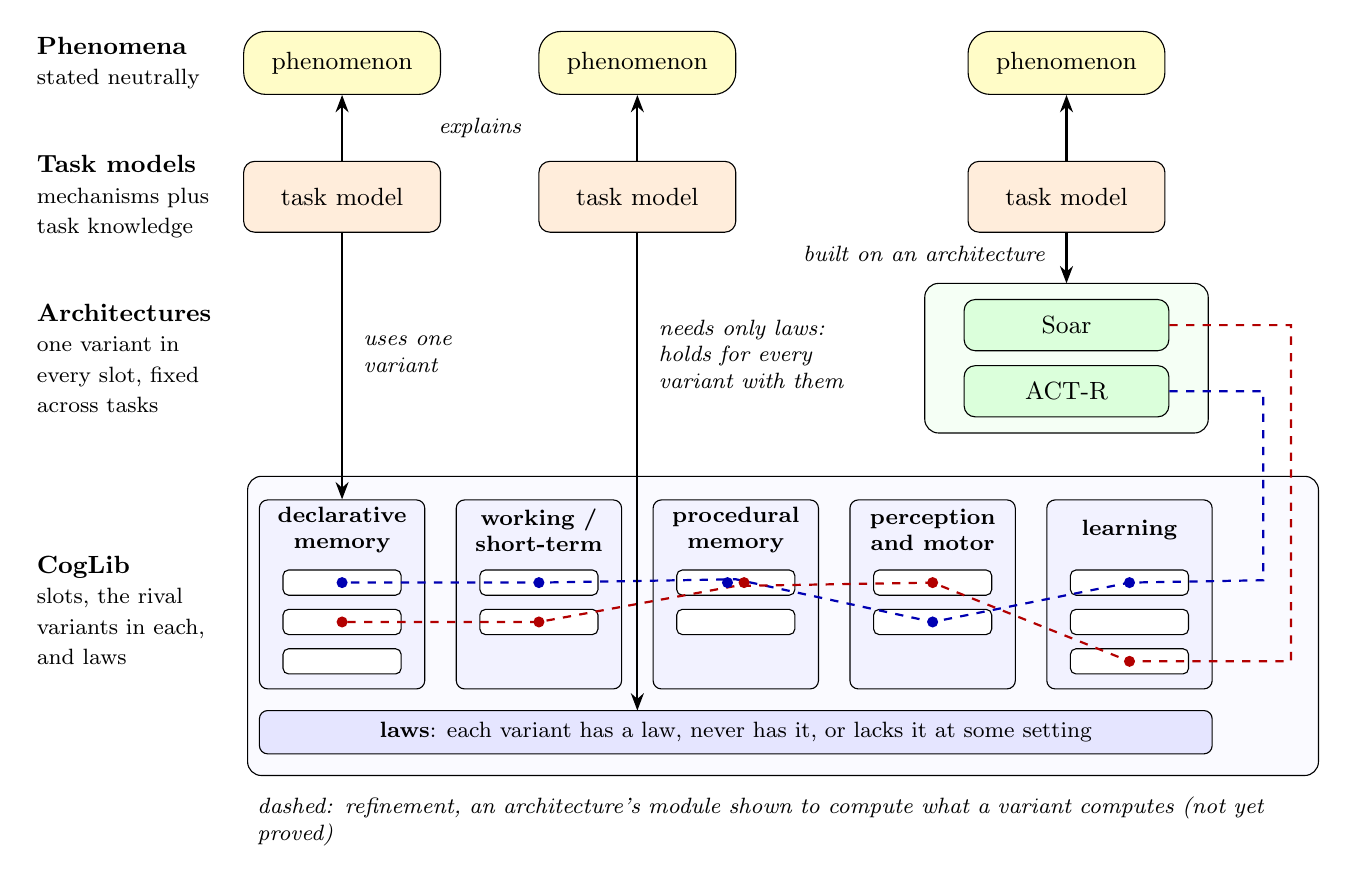
\begin{tikzpicture}[
  font=\small,
  lay/.style={font=\small, align=flush left, text width=2.45cm, anchor=west},
  slot/.style={draw, rounded corners=3pt, fill=blue!5, minimum width=2.1cm, minimum height=2.4cm},
  slottitle/.style={font=\footnotesize\bfseries, align=center, text width=2.0cm},
  card/.style={draw, rounded corners=2pt, fill=white, minimum width=1.5cm, minimum height=0.32cm},
  model/.style={draw, rounded corners, fill=orange!14, align=center, minimum width=2.5cm, minimum height=0.9cm},
  phen/.style={draw, rounded corners=8pt, fill=yellow!22, align=center, minimum width=2.5cm, minimum height=0.8cm},
  arch/.style={draw, rounded corners, fill=green!14, align=center, minimum width=2.6cm, minimum height=0.65cm},
  arr/.style={-{Stealth[length=2.2mm]}, thick},
  note/.style={font=\footnotesize\itshape, align=left, anchor=west}
]
% ---------- CogLib ----------
\draw[rounded corners=5pt, fill=blue!2] (2.8,-0.6) rectangle (16.4,3.2);
\foreach \x/\ttl/\n [count=\i] in {4.0/{declarative\\memory}/3, 6.5/{working /\\short-term}/2,
     9.0/{procedural\\memory}/2, 11.5/{perception\\and motor}/2, 14.0/{learning}/3} {
  \node[slot] (s\i) at (\x,1.7) {};
  \node[slottitle] at (\x,2.52) {\ttl};
  \foreach \r in {1,...,\n} { \node[card] (c\i-\r) at (\x,2.35-0.5*\r) {}; }
}
\node[draw, rounded corners=3pt, fill=blue!10, minimum width=12.1cm, minimum height=0.55cm,
      font=\footnotesize] (laws) at (9.0,-0.05)
  {\textbf{laws}: each variant has a law, never has it, or lacks it at some setting};
% ---------- Architectures ----------
\draw[rounded corners=5pt, fill=green!4] (11.4,3.75) rectangle (15.0,5.65);
\node[arch] (soar) at (13.2,5.12) {Soar};
\node[arch] (actr) at (13.2,4.28) {ACT-R};
% threads: one variant per slot (dashed = refinement, to be proved)
\draw[dashed, thick, blue!70!black]
  (actr.east) -- (15.7,4.28) -- (15.7,1.88) -- (c5-1.center) -- (c4-2.center) --
  ([yshift=1.2pt]c3-1.center) -- (c2-1.center) -- (c1-1.center);
\draw[dashed, thick, red!70!black]
  (soar.east) -- (16.05,5.12) -- (16.05,0.85) -- (c5-3.center) -- (c4-1.center) --
  ([yshift=-1.2pt]c3-1.center) -- (c2-2.center) -- (c1-2.center);
\foreach \c in {c5-1,c4-2,c2-1,c1-1} \fill[blue!70!black] (\c.center) circle (2pt);
\foreach \c in {c5-3,c4-1,c2-2,c1-2} \fill[red!70!black] (\c.center) circle (2pt);
\fill[blue!70!black] ([xshift=-3pt]c3-1.center) circle (2pt);
\fill[red!70!black] ([xshift=3pt]c3-1.center) circle (2pt);
% ---------- Task models and phenomena ----------
\node[model] (m1) at (4.0,6.75) {task model};
\node[model] (m2) at (7.75,6.75) {task model};
\node[model] (m3) at (13.2,6.75) {task model};
\foreach \i in {1,2,3} {
  \node[phen] (p\i) at (m\i |- 0,8.45) {phenomenon};
  \draw[arr] (m\i.north) -- (p\i.south);
}
\draw[arr] (m1.south) -- (s1.north);
\draw[arr] (m2.south) -- (7.75,0.225);
\draw[arr] (m3.south) -- (13.2,5.65);
\node[note] at (4.15,4.75) {uses one\\variant};
\node[note] at (7.9,4.75) {needs only laws:\\holds for every\\variant with them};
\node[note, anchor=east, align=right] at (13.05,6.02) {built on an architecture};
\node[font=\footnotesize\itshape] at (5.75,7.62) {explains};
% ---------- Layer labels ----------
\node[lay] at (0,8.45) {\textbf{Phenomena}\\{\footnotesize stated neutrally}};
\node[lay] at (0,6.75) {\textbf{Task models}\\{\footnotesize mechanisms plus task knowledge}};
\node[lay] at (0,4.7) {\textbf{Architectures}\\{\footnotesize one variant in every slot, fixed across tasks}};
\node[lay] at (0,1.5) {\textbf{CogLib}\\{\footnotesize slots, the rival variants in each, and laws}};
\node[font=\footnotesize\itshape, anchor=north west, align=left, text width=13.3cm] at (2.8,-0.75)
  {dashed: refinement, an architecture's module shown to compute what a variant computes (not yet proved)};
\end{tikzpicture}
\caption{How CogLean is meant to be organized. \textbf{CogLib} is a set of
slots, the kinds of memory and process that the Common Model of
Cognition distinguishes, and ``memory'' is not one of them but several.
Each slot holds rival variants behind one interface (discrimination
nets and activation-based retrieval, for example, are two variants of
declarative memory), and each law is something a variant provably has,
never has, or lacks at some setting. An \textbf{architecture} is one
variant chosen in every slot and held fixed across tasks; Soar and
ACT-R share the slots and differ in what fills them. A \textbf{task
model} adds task knowledge and explains a phenomenon. It may use one
variant (EPAM, the strategy-choice model), require only laws and so
hold for every variant that has them (the confident errors of
multi-digit addition), or be built on an architecture (the models that
run on the Lean ACT-R and Soar). The figure shows the intended
organization and not the present state: CogLib so far has rival
variants only for long-term associative memory, the other slots are
filled in the architecture specifications, and the dashed links between
the two are the refinement theorems still to be proved.}
\label{fig:arch}
\end{figure}
\clearpage

\bibliographystyle{unsrtnat}
\bibliography{refs}

\end{document}
